% sdd.tex

\documentclass{report}
\linespread{1.2}
\renewcommand{\chaptername}{}
\usepackage{times} %Times is nice
\usepackage{url}
\usepackage[T1]{fontenc}
\usepackage{titlesec, blindtext, color}
\usepackage{amsmath}
\usepackage{graphicx}
\usepackage{hyperref}
\usepackage{float}

\definecolor{gray75}{gray}{0.75}
\newcommand{\hsp}{\hspace{20pt}}
\titleformat{\chapter}[hang]{\Huge\bfseries}{\thechapter\hsp\textcolor{gray75}{|}\hsp}{0pt}{\Huge\bfseries}

\begin{document}

\title{System Design Document for Barcode Scanner Project (SDD) - Group 30}
\author{
    Christian Svensson\\
    \and
    Olle Andreasson\\
    \and
    Olof Karlsson\\
    \and
    Rasmus Letterkrantz
}
\date{\today}
\maketitle

\tableofcontents

\chapter{Introduction}

\section{Design Goals}
Our goal with the structure of our code is to keep the database, the algorithm for analyzing an image and the android specific GUI, separated from each other so that each and every one of these parts can be exchanged or updated without affecting the performance of the other. 
The way that Android applies MVC\cite{website:mvc} is that it forces you to create an Activity for each view you want to display. Each activity requires an accompanying XML file. The XML file defines the user interface and the Activity is the controller for that view. The only way to add data to this is by adding you own (Java) code and forwarding that data to the controller. In other words, MVC is applied for each new view you create for your application.

\pagebreak

\section{Definitions, Acronyms and Abbreviations}

\begin{itemize}
    \item{GUI}, Graphical User Interface.
    \item{Android}, open source operating system for mobile units (smart-phones, tablets, etc).
    \item{Java}, platform independent programming language.
    \item{XML}, Extensible Markup Language is used for structuring the elements in the GUI.
    \item{SQLite}, the database used to store the barcodes.
    \item{Locator}, class used to locate the barcode on a given image.
    \item{Generator}, class used for analyzing the pattern extracted by the Locator and generating the actual key.
    \item{MVC}, a way of partition an application with a GUI into distinct parts avoiding a mixture of GUI-code, application code and data spread all over.
\end{itemize}

\chapter{System Design}

\section{Overview}
The application will strive to keep a MVC way of structuring the code but as the standards for programming Android have a very unique way separating views and data this will be more reflected in the functionality rather than the visual appearance of the code.

\subsection{The Model Functionality}
CameraActivity's interface will be the main entry for our model functionality. From there the different functionality parts of our model can be called and then presented in other, separated views.

\subsection{Storage}
Each barcode will be stored in a SQLite database as a product. The barcode itself will be used as the identifier of the product and the price, description and name of the product will be stored along with it. The database will be using a single table and view called Products and ProductsView, respectively.

\pagebreak

\section{Software Decomposition}

\subsection{General}

The application is decomposed into the following parts:

\begin{itemize}
  \item{camera}, contains the CameraActivity and a helper class to the camera.
  \item{activities}, contains all the other activities.
  \item{core}, contains all of our logic (the barcode scanning algorithm).
  \item{database}, contains all classes that handle the database.
\end{itemize}

\subsection{Decomposition into subsystems}
The only subsystems in the application is the DatabaseHandle which writes and reads to/from the database, and the camera which is used to take an image. 

\subsection{Layering}
On our highest level we have the views that are displayed on the screen. Following those we have the activities which are controlling what the views are going to display. On our lowest layer we have the core logic (analyzer, DatabaseHelper, etc) which is read by the activities.

\subsection{Dependency analysis}
The dependencies that exists are shown in diagram below. All other dependencies not listed are the ones between Activity -> View and Activity -> Model; in other words the fact that the Activity needs the data from the model and the view to display the data on from the interface.

\begin{figure}[H]
		\centering
		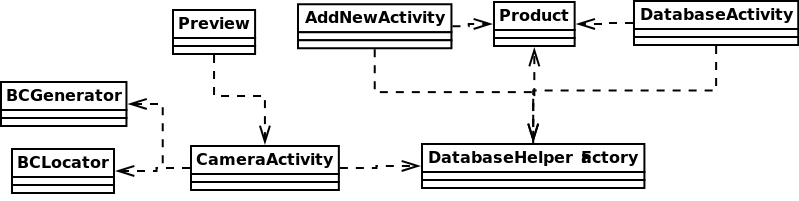
\includegraphics[width=\textwidth]{dependencydiagram.png}
		\caption{Dependency Diagram}
		\label{fig:Dependency Diagram}
\end{figure}

\begin{figure}[H]
		\centering
		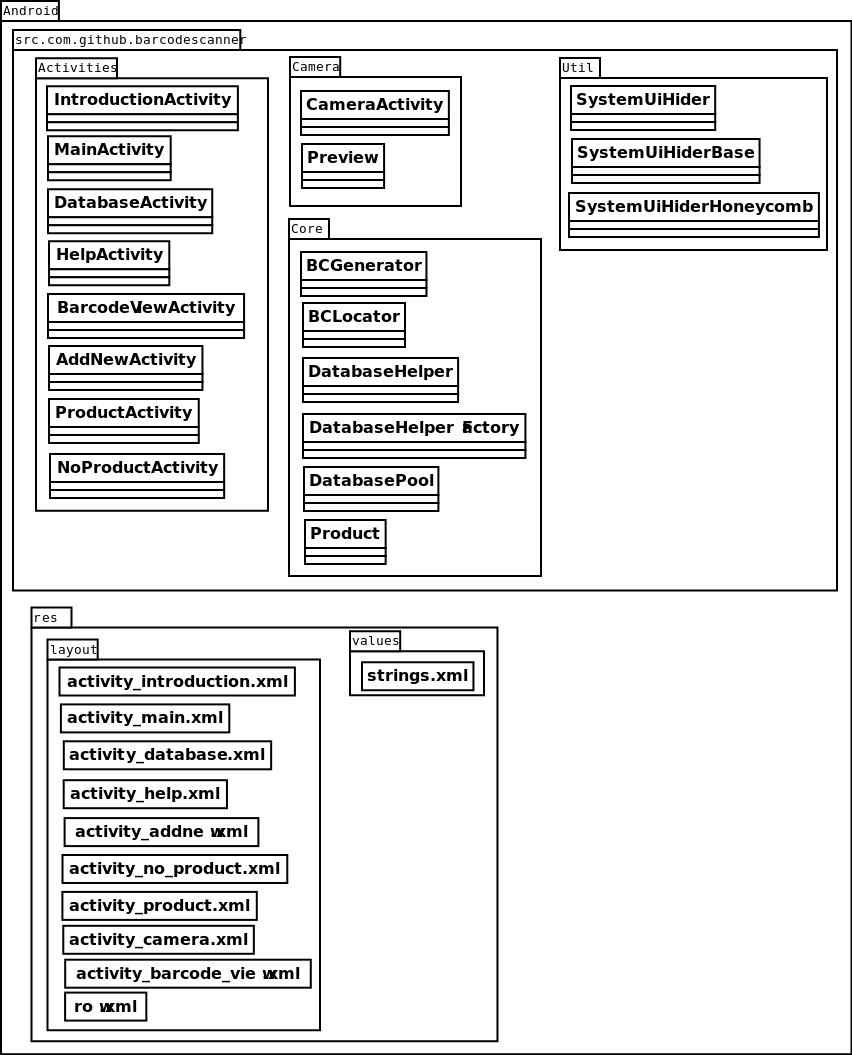
\includegraphics[width=\textwidth]{packagediagram.png}
		\caption{Package Diagram}
		\label{fig:Package Diagram}
\end{figure}

\pagebreak

\section{Concurrency Issues}
NA. The application is only tied to one mobile unit, meaning that only one instance of the application will run at once and each activity uses distinct, separate instructions for performing a task. The database is also only tied to one mobile unit. All together the application never performs any concurrent task that can interfere with another instruction in a harmful way. 


\section{Access control and security}
NA

\section{Boundary conditions}
The application can only be run on mobile units running Android 4.0+.

\bibliographystyle{plain}
\bibliography{referencessdd.bib}

\appendix

\pagebreak

\begin{figure}[H]
		\centering
		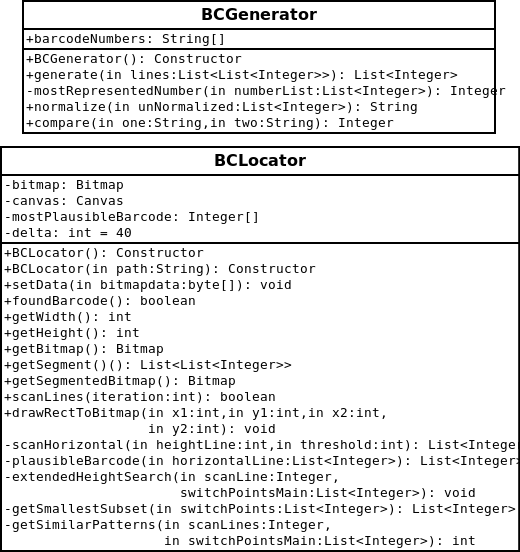
\includegraphics[width=\textwidth]{classdiagramcore.png}
		\caption{Class Diagram}
		\label{fig:Class Diagram for Core package.}
\end{figure}

\pagebreak

\begin{figure}[H]
		\centering
		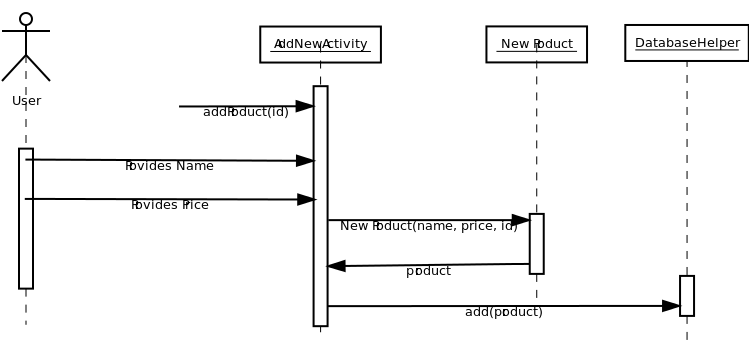
\includegraphics[width=\textwidth]{sequencediagram.png}
		\caption{Sequence Diagram for adding a product to the database}
		\label{fig:Sequence Diagram 1}
\end{figure}

\begin{figure}[H]
		\centering
		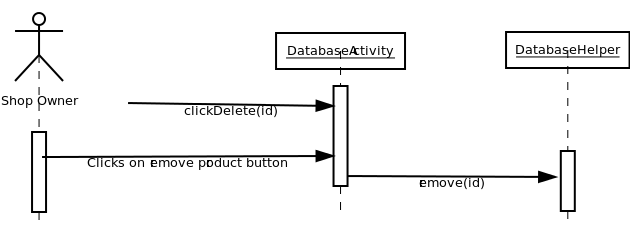
\includegraphics[width=\textwidth]{sequencediagram2.png}
		\caption{Sequence Diagram for removing a product from the database}
		\label{fig:Sequence Diagram 2}
\end{figure}

\end{document}
